\documentclass[11pt, a4paper]{article}
\usepackage{alicetex}
\usepackage{parskip}
\lstset{style=defaultstyle}

\title{General Assignment Template}
\author{Leo Duncan \\ ldun202, 657579290}
\date{xxth Month 202x}

\begin{document}

\maketitle

\section{General Math}
\quest{Basic math examples for convenient copy-pasting}

\subsection{(a)} %Basic multiline equation
\quest{Basic multiline equation example.}

\begin{equation*}
    \begin{split}
        a &= b + c \\
        &= (b + d) - (d - c) \\
    \end{split}
\end{equation*}

\subsection{(b)} %Vectors and matrices
\quest{Vectors and matrices.}

Column vector square brackets: $\bm{x} = \colvec{1\\2\\3}$, round brackets: $\vec{v} = \colvecbr{4\\5\\6\\7}$.

Column vector square brackets: $\bm{u} = \colvec{1&2&3}$;

Round brackets: $\vec{w} = \colvecbr{4&5&6&7}$.

Matrix $A = \left[\begin{array}{cccc}
    a & b & c & d \\
    e & f & g & h \\
    i & j & k & l \\
\end{array}\right]$.

Another example $B = \left[\begin{array}{ccc|c}
    a & b & c & d \\
    e & f & g & h \\
    i & j & k & l \\
\end{array}\right]$.

\subsection{(c)} %Sums, limits, integration
\quest{Sums, limits, integration}

$$\sum \frac{1}{k+\sqrt{k}}$$

$$\sum\limits_{k=2}^\infty \frac{3^k-1}{4^k}$$

$$\lim_{k \to \infty} \frac{k^2 + k + 1}{2k^2}$$

$$\int_{-1}^{1} e^{x} \, dx$$

\subsection{(d)} %Using /frac and /dfrac
\quest{Using \textbackslash \texttt{frac} and \textbackslash \texttt{dfrac}.}

Using \textbackslash \texttt{frac} $\frac{k^2+1}{k^3+1}$ and now using \textbackslash \texttt{dfrac} $\dfrac{k^2+1}{k^3+1}$.

Note that when in "big" equation environment, \$\$, they give the same result. Avoid using \textbackslash \texttt{dfrac} unless necessary.
\newpage


\section{Graphics}
\quest{Pictures and everything so exciting}

Heres an example of two images side-by-side.

\begin{figure}[!h]
    \begin{subfigure}[b]{0.45\textwidth}
      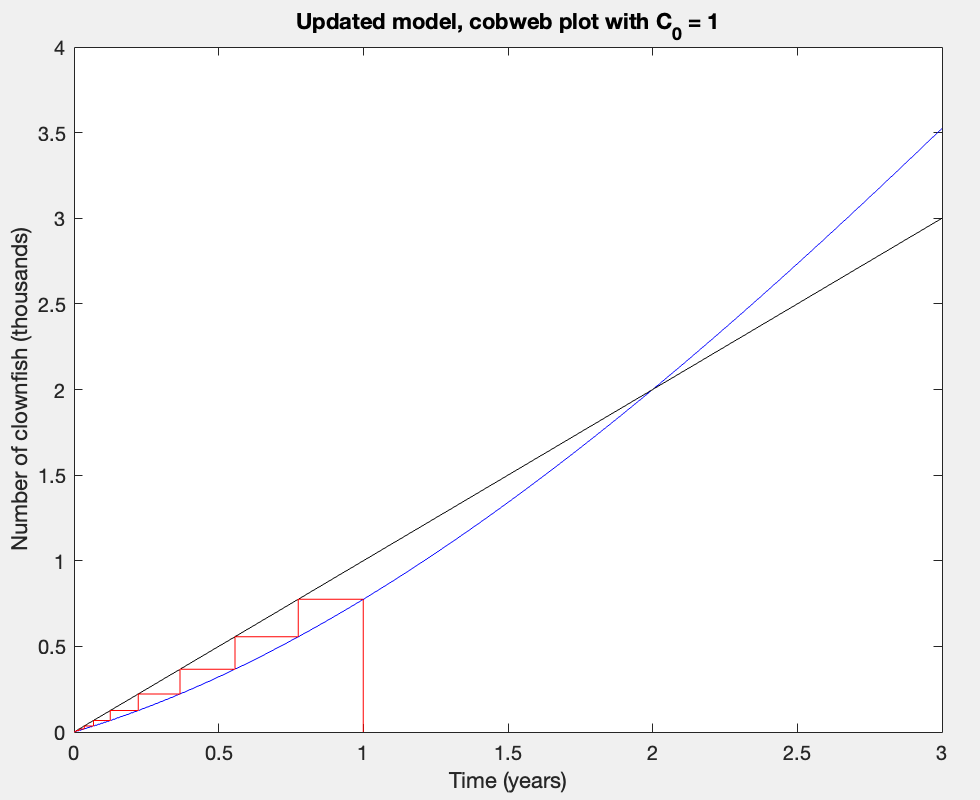
\includegraphics[width=\textwidth]{images/clownfishplot2.png}
      \label{fig:f6}
      \caption{Cobweb plot $C_0 = 1$}
    \end{subfigure}
    \hfill
    \begin{subfigure}[b]{0.45\textwidth}
      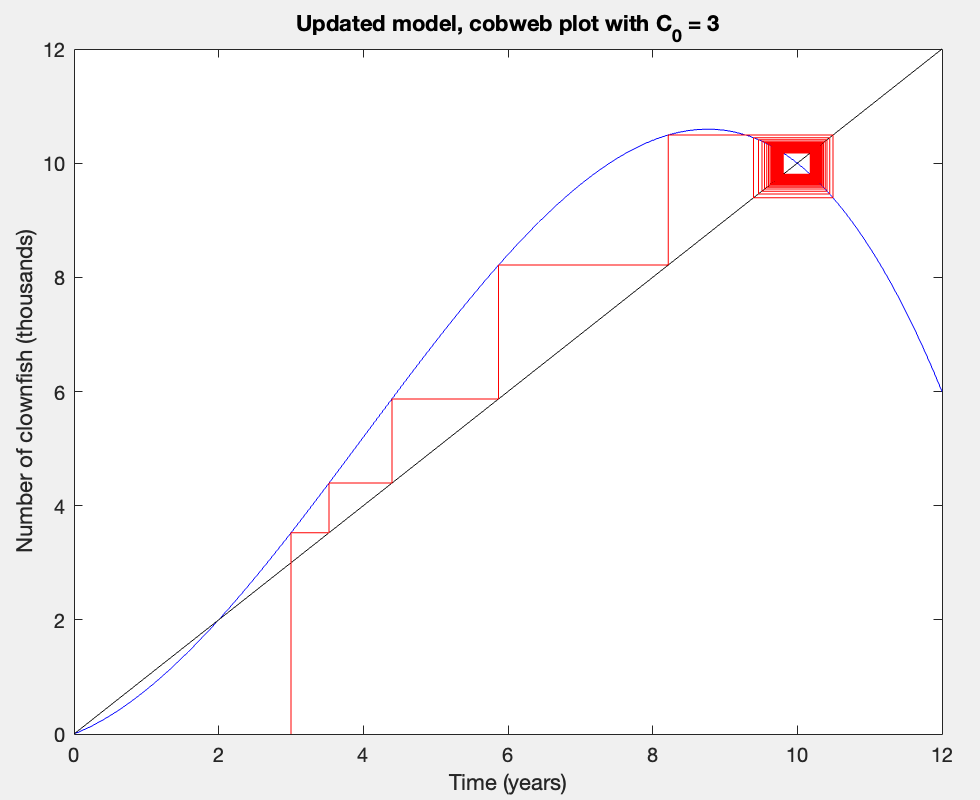
\includegraphics[width=\textwidth]{images/clownfishplot3.png}
      \label{fig:f7}
      \caption{Cobweb plot $C_0 = 3$}
    \end{subfigure}
    \caption{Updated model cobweb plots.}
\end{figure}




\section{Tables}
\quest{Yep, tables, as the title would suggest}



\section{Code}
\quest{Code code code code code}
%be sure to include pseudocode examples too (220 ass 1)

\begin{lstlisting}[language=MATLAB]
Seq = randi(2,1,1000); % generate random sequence of coin flips
k = 0;

% while-loop that runs until the desired sequence, THH, is found
while(Seq(k+1)~=2 || Seq(k+2)~=1 || Seq(k+3)~=1)
    k = k + 1;
end

disp(k) % output how many flips before the sequence THH
\end{lstlisting}




%ACTUALLY MAYBE PUT THESE FINAL TWO IN A SEPEATE FILE (MAYBE COMBINE WHEN DONE)
\section{Academic Writing}
\quest{How to format big chunks of writing}




\section{Bibliography}
\quest{Referencing, footnotes, etc}





\end{document}